\documentclass[11pt]{article}
\usepackage[utf8]{inputenc}

\title{Generative Adversarial Networks}
\author{Jacob Smith}
\date{December 5, 2017}

\usepackage{natbib}
\usepackage{graphicx}
\usepackage{bm}
\usepackage[options ]{algorithm2e}
\usepackage{parskip}

\graphicspath{{./img/}}

\begin{document}
\maketitle

\begin{abstract}
    Deep generative networks have often fallen short, especial when compared to discriminative models. Since their conception in 2014, generative adversarial networks have seen exponential growth in research. These networks offer promising results for both unsupervised learning and generative models. This research paper presents an overview of generative adversarial networks. Specifically, we will examine the motivation behind GANs, their theoretical justification, the current state of GANs and the research frontiers that have yet to be explored.
\end{abstract}

\section{Introduction}
Deep learning have made astounding progress within the past decade. Discriminative models have recently surpassed the abilities of human within the domain of pattern recognition \citep{2014arXiv1404.7828S}. These successes can attributed to vast, high dimension datasets in conjunction with large neural networks using linear activation functions, dropout regularization techniques and backpropagation to update the parameters \citep{2014arXiv1406.2661G}. However, deep learning possesses many more ambitious goals. Until recently, success has mostly been seen with supervised classifiers; however, deep generative models now competitively rival their discriminative counterparts.

Generative models learn the joint probability distribution $p(x,y)$ of an input $x$ and label $y$ whereas discriminative models directly learn the conditional probability $p(y|x)$. Generative models may be used as classifiers using Bayes rules to calculate the conditional probability $p(x,y)$ which can then be used to make predictions \citep{NIPS2001_2020}. Depending on the model, knowledge of the probability distribution can be created both explicitly and implicitly \citep{Goodfellow-et-al-2016}. Those which do not directly model a probability distribution offer mechanisms which require implicit knowledge of the underlying distribution, such as creating a sample from that distribution \citep{Goodfellow-et-al-2016}. As humans, we are able to understand the world around us with tremendous precision. It is easy to underestimate the complexity of the data we process to accomplish this feat. Although progress within the machine learning field is rapidly advancing, computers still have limited understanding of the data the process. Generative models, especially deep generative models, offer promising results towards this goal \citep{genmodelingopenai}.

\begin{figure}
\centering
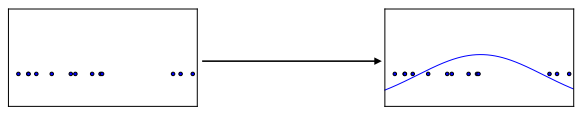
\includegraphics[scale=0.7]{pdf}
\caption{The process density estimation of one-dimensional data and a Gaussian distribution \citep{2017arXiv170100160G}. Generative models take a dataset $D$, sourced from a distribution $p_{data}$, a create an estimate of that distribution $p_{model}$.}
\label{fig:pdf}
\end{figure}

The process of training a generative model is very similar to a discriminative model. Using large amounts of data collected from a specific domain, we train the model to generate data from that domain. As these models have fewer parameters than that the number of data samples, they are forced to internalize some representation of the data. Although, unlike supervised training, there exists no explicit desired output. The problem becomes defining a cost function which forces the generative model to produce data more like that of the domain.

Generative adversarial networks (GANs), first introduced in 2014, offer a new framework for estimating generative models with use of an adversarial process \citep{2014arXiv1406.2661G}. These models offer a clever approach to solving the aforementioned problem of explicitly defining a cost function. Rather than training a single model, a discriminator is introduced. These two networks are pitted against each other in a minimax game. The generative model $G$ attempts to produce data that resembles that of the training set while the discriminative model $D$ attempts to classify whether or not a sample was real of generated. To train this network, $G$ attempts to maximize the error rate of $D$ whereas $D$ attempts to minimize it. The goal of the GAN algorithm is to reduce the distance between the data and generated probability distributions. Backpropagation is used to update the parameters and to train each model. In the ideal case, $D$ is unable to distinguish the generated samples from the real samples and produces an error rate of $\frac{1}{2}$ \citep{2014arXiv1406.2661G}.

\section{Motivations}
There exists several compelling reasons for studying generative modeling \citep{2017arXiv170100160G}. These models are extremely useful when your goal is understand the underlying distribution parameters. For example, joint probability distributions of high dimensional data is relevant to both applied math and engineering \citep{2017arXiv170100160G}. Generative models are also applicable to reinforcement learning, particularly model-based learning algorithms. A time series generative model, one which predicts future states of an environment given the current state of the environment and an agents actions, are of particular interest \citep{2017arXiv170100160G}. An agent may learn the best action to take in a given scenario by querying this generative model and choosing the one which outputs the best state of the world. Furthermore, generative models, especially GANs, have recently excelled at semi-supervised learning.

Proposed in the original GAN paper \citep{2014arXiv1406.2661G}, semi-supervised techniques used in conjunction with GANs have recently proven themselves as a reputable technique. The premise involves training the discriminator to classify images into $n + 1$ classes where $n$ is the number of class labels and the additional $1$ is the class of a fake image. This algorithm is able to obtain great performance on relatively small labeled datasets when compared to labeled datasets typically state of the art supervised algorithms \citep{2017arXiv170100160G}. Currently, the best performing semi-supervised GAN are feature matching GANs, where the new objective of the generative model is to minimize the distance between a layer $l$ of the discriminator \citep{2016arXiv160603498S}.

Many applications require multi-modal outputs. For example, predicting the next action of a self-driving car. Within this context, it is important the model not be trained by traditional methods, such as using mean squared error to minimize the distance between the expected and predicted actions. These models cannot be used in situations where there is more than one appropriate prediction. Generative modeling, especially GAN, allow machine learning to function the scenarios where one input corresponds to multiple acceptable outputs \citep{2017arXiv170100160G}.

Tasks which involve image generation, modification or translation are all highly applicable to generative models. Although GANs may be used to generate any type of data, images remain the most commonly used source of training data. Research conducted within the past three years demonstrates the capabilities of GANs to perform these tasks \citep{2017arXiv170100160G, 2016arXiv161102200T, 2014arXiv1411.1784M}. For example, GANs have recently been shown to be capable of translating aerial photographs into maps and sketches into realistic images \citep{2017arXiv170100160G}.

When compared to other generative models, especially deep generative models, GANs possess several advantages... quicker? no Markov chains?

\begin{figure}
\centering
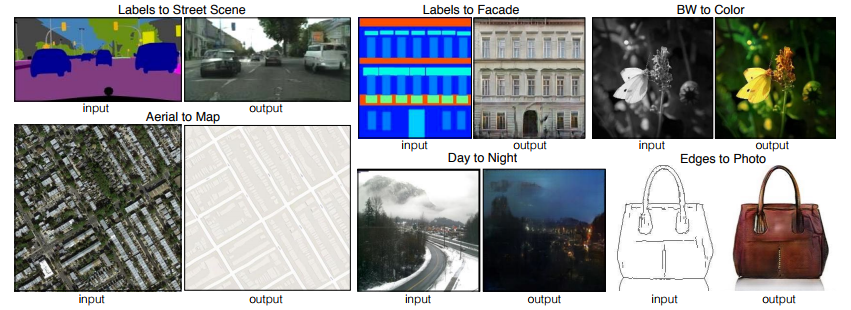
\includegraphics[scale=0.55]{img2img}
\caption{Examples of the image-to-image technique developed by Isola \textit{et al.} \citep{2016arXiv161107004I}. This technique makes use of conditional generative adversarial networks to map across image domains.}
\label{fig:Image to Image Examples}
\end{figure}

\section{Background}
Generative adversarial networks may use any differentiable functions for the models; however, the optimal results are typically achieved when neural networks are used \citep{2014arXiv1406.2661G}. We first define a vector $z$ such that $z~p_z(z)$. This vector becomes the argument of the generator $G(z;\theta_g)$ where $G$ is a differentiable function and $\theta_g$ is its parameters. Another differentiable function $D(x;\theta_d)$ for the discriminator. This function takes as input a vector $x$, either from the output of $G$ or a sample from the training set, and is parametrized by $\theta_d$. The output of the discriminator is a scalar number representation the probability that the arguments were derived from the training data. In this situation, there exists a minimax game where $D$ attempts to maximize the probability of assigning a correct label and $G$ attempts to minimize $\log(1-D(G(z)))$. The networks $G$ and $D$ play a minimax game with the value function $V(D,G)$:

$$\min_{G}\max_{D}V(D, G) = \mathbb{E}_{x\sim p_{data}(x)}\Big[\log(D(x))\Big] + \mathbb{E}_{z\sim p_z(z)}\Big[\log(1-D(G(z)))\Big]$$

For the training step, any variant of gradient descent may be used with respect to the individual cost functions \citep{2017arXiv170100160G}. The first updates $\theta_D$ while attempting to minimize the discriminator cost function $J_D$ while the other updates $\theta_G$ while attempting to minimize the generator cost function $J_G$. There exist several variations of the cost function that may be used for training purposes; however, the discriminator cost has remained the same for each.

$$J^{(D)}(\theta_D,\theta\G) = -\frac{1}{2}\mathbb{E}_{x\sim p_{data}(x)}\Big[\log(D(x))\Big] - \frac{1}{2}\mathbb{E}_{z\sim p_{z}(z)}\Big[\log(1-D(G(z)))\Big]$$

This is a standard cross entropy cost function that is trained on two minibatches, one from the dataset and one from the generator. For this to become a zero-sum game, the cost function of the generator is simply the negation of the discriminator.

$$J^{(G)}(\theta_D,\theta\G) = -J_d(\theta_D,\theta\G)$$

This version of the generator loss function is particularly useful for theoretical analysis as shown in the first GAN paper \citep{2014arXiv1406.2661G}. Goodfellow demonstrated that the minimax game is the same as minimizing the Jensen-Shannon divergence and that each player will eventually converge if both players are able to directly update the function space as oppose to the parameters within the network \citep{2017arXiv170100160G}. However, in this minimax version, the loss function of the generator suffers from a vanishing gradient when the discriminator confidently rejects the generated data. The solution proposed by Goodfellow is to train the generator to maximize $log(D(G(z)))$ rather than minimize $log(1-D(G(z)))$ \citep{2014arXiv1406.2661G}. This function is heuristically motivated as to provide strong gradients when either the generator or discriminator is not functioning optimally. In this version, the generator attempts to maximize the log probability of a misclassification whereas the minimax version attempts to minimize the log probability of the discriminator being correct.

$$J^{(G)}(\theta_D,\theta\G) = -\frac{1}{2}\mathbb{E}_{z\sim p_{z}(z)}\Big[\log(D(G(z)))\Big]$$

A maximum likelihood cost is another option for training GANs \citep{2017arXiv170100160G}. It can be shown that that this cost function minimizes the Kullback-Leibler divergence between $p_{data}$ and $p_{model}$ instead of the Jensen-Shannon divergence. This cost estimator is useful as it allows for comparison with other generative models; however, it behaves similarly to the minimax cost function as seen in \ref{fig:CostFunc}.

$$J^{(G)}(\theta_D,\theta\G) = -\frac{1}{2}\mathbb{E}_{z\sim p_{z}(z)}\Big[\exp(\sigma^{-1}(D(G(z))))\Big]$$

\begin{figure}
\centering
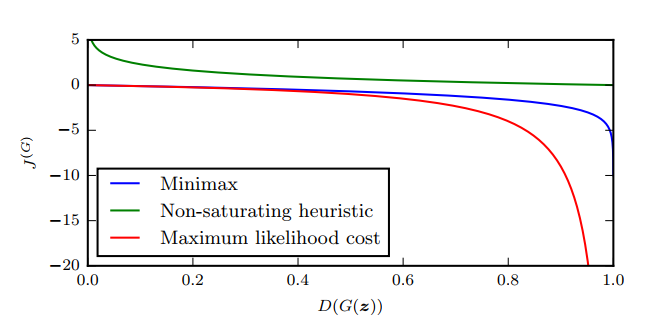
\includegraphics[scale=0.5]{costfunc}
\caption{A comparison of the generator cost function for generative adversarial networks. When $D(G(z))$ is close to $0$, the gradient is saturated for both the minimax and maximum likelihood cost functions. This situation occurs when the discriminator $D$ confidently rejects the generated value $G(z)$ as fake. Therefore, the non-saturated heuristic cost function is the only one which works well in practice. Furthermore, the maximum likelihood cost function may produce high variance due to the rapid decrease as $D(G(z))$ nears $1$. Image retrieved from Goodfellow NIPs tutorial \citep{2017arXiv170100160G}.}
\label{fig:CostFunc}
\end{figure}

This following algorithm presents initial training algorithm used by Goodfellow \textit{et al.} when GANs were introduced in 2014 \citep{2014arXiv1406.2661G}. Many modifications have been made by various sources. The first step in the algorithm is to optimize the discriminator $D$. Initially, many thought it would be optimal to train $D$ to completion; however, as previously mentioned, this is still a controversial topic among researchers \citep{2017arXiv170100160G}. For the initial GAN experiments, this number was set to $1$ to reduce computation time.

\begin{algorithm}[H]
  \SetAlgoLined
  \Input{$n$: The number of training iterations} \linebreak
  \Input{$k$: The number of discriminator iterations} \linebreak
  \For{training iteration in n} {
    \For{discriminator iteration in k} {
      sample $m$ vectors $\{z^{(1)},...,z^{(m)}\}$ from distribution $p_z(z)$\;
      sample $m$ vectors $\{x^{(1)},...,x^{(m)}\}$ from the training samples\;
      update the discriminator using its stochastic gradient
      $$\nabla_{\theta_d}\frac{1}{m}\sum_{i=1}^{m}[\log(D(x^{(i)}))+\log(1-D(G(z^{(i)})))]$$
    }
    sample $m$ vectors $\{z^{(1)},...,z^{(m)}\}$ from distribution $p_z(z)$\;
    update the generator using its stochastic gradient\;
    $$\nabla_{\theta_g}\frac{1}{m}\sum_{i=1}^{m}[\log(1-D(G(z^{(i)})))]$$
  }
  \caption{The initial generative adversarial network algorithm developed by Goodfellow \textit{et al.} in 2014 \citep{2014arXiv1406.2661G}. Multiple variations of this algorithm have since been produced. One of the benefits of adversarial networks is that they may be updated using back propogation.}
\end{algorithm}

\section{Issues}
There exist several issues that characterize generative adversarial networks. Some are related design of GANs or their underlying network implementations. These issues lay at the forefront of GAN research.

\subsection{Instability}
Generative adversarial networks are often characterized by their instability \citep{2017arXiv170100160G}. The training process makes use of gradient descent which does not guarantee convergence to the Nash equilibrium, the game theory equilibrium that involves two competing players. This is different than network optimization which is common in discriminative models. When each network trains, even if the specified network improves, the other may regress. This sometimes leads to the scenario where each network repeatedly undo's the other's progress. This problem is not specific to GANs, but to any game situations \citep{2017arXiv170100160G}. It was shown in the first paper that convergence was guaranteed if updates could be made to the function space, but no theoretical justification was been found that guarantees convergence within the parameter space \citep{2014arXiv1406.2661G}. However, there is no theoretical proof that that these games should not converge \citep{2017arXiv170100160G}. Typically, adversarial networks often oscillate between different kinds of samples without converging to an equilibrium in a phenomenon called mode collapse.

\subsection{Mode Collapse}
Mode collapse occurs when the generator collapses several different latent space vectors $z$ map to the same outputs. Full mode collapse is rare; however, partial mode collapse always occurs and varies by intensity. For example, the generator may create two images that only differ by colour but were generated with very different latent vectors. This occurs when the capacity of the generator is superior to that of the discriminator. Backpropagation does not necessarily follow the minimax game mentioned earlier and may behave like the maximin version.

$$G^* = \max_{D}\min_{G}V(F, D)$$

When this occurs, the generator attempts to map every latent vector to the one $x$ variable the discriminator is most likely to guess is real. When training, one can only hope the behavior resembles the minimax version. It is often speculated that the root cause of the issue the particular divergence measure used. Specifically, it is often asserted that mode collapse is caused by the use of Jensen-Shannon divergence; however, the use of Kullback-Leibler divergence has be shown to worsen the problem \citep{2017arXiv170100160G}. As mode collapse is currently an unavoidable reality for GANs, their applications are limited to situations where it is acceptable to generate only a small number of distant samples \citep{2017arXiv170100160G}. A potential solution to this problem is discussed in the following section.

\begin{figure}
\centering
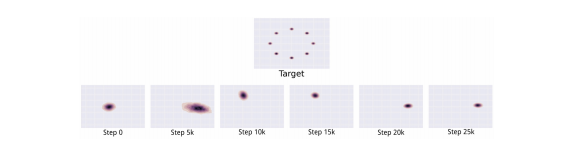
\includegraphics[scale=0.8]{modecollapse}
\caption{An example of mode collapse as demonstrated by Metz \textit{et al.} \citep{2016arXiv161102163M}. The generated samples cluster around only one of the modes and do not spread out as they should. Throughout the training process, this cycle continues does not reach an equilibrium.}
\label{fig:Mode Collapse Example}
\end{figure}

\subsection{Image Quality}
When generating images, problems often arise due to the generators difficulties with perspective, counting and structure \citep{2017arXiv170100160G}. For example, an generated animal may not have a 3D structure, have misplaced limbs or have too many of a specific body part. These issues arise due to the underlying model architecture and are not an inherent problem the adversarial network. Furthermore, generated image resolution has remained relatively low; however, recent improvements outlined in the following section show improvements with regard to resolution \citep{2017arXiv171010196K}.

\subsection{Evaluation}
The evaluation procedure for generative adversarial networks remains an open debate as there exist no clear quantitative measurement to evaluate the models \citep{2017arXiv170100160G}. For example, models with high likelihood may produce poor samples and models with low likelihood may produce realistic samples. Several variations of the GANs examine the tradeoffs of divergence measures other than the original Kullback-Leibler divergence \citep{2015arXiv151101844T}. It can be shown that different metrics favor different models. Therefore, it is important to asses one's model within the context of the whole application \citep{2015arXiv151101844T}.

\subsection{Discrete Data}
GANs assume a model implementation that is differentiable due to it's use of back propagation. Therefore, this restricts their ability to generate discrete data. Goodfellow proposes several solutions such as algorithm modifications, discretization and the use of concrete distributions or Gumbel-softmax \citep{2017arXiv170100160G}.

\section{Training Improvements}
A substantial amount of research has been conducted within the past three years with regards to improving GAN training procedures. A paper released by Goodfellow approximately one year after the debut of GANs outlines several techniques that can be applied to improve the training process \citep{2016arXiv160603498S}. As previously mentioned, the optimal solution for GANs remains convergence of the Nash equilibrium of the minimax game; however, gradient descent attempts to find a local minima. The following techniques introduced by Goodfellow \textit{et al.} address the instability of GANs and attempt to increase the probability of convergence.

\subsection{Feature Matching}
Feature matching involves the definition of a new cost function for GANs such that they do not overtrain on the current discriminator \citep{2016arXiv160603498S}. Instead of optimizing on the output of the discriminator, the new objective requires the generator to minimize the difference between the expected value on some intermediate layer. The objective function can be described as $\Big|\Big|\mathbb{E}_{x\sim p_{data}(x)}\Big[f(x)\Big] - \mathbb{E}_{z\sim p_{z}(z)}\Big[f(G(z))\Big]\Big|\Big|_2^2$ where $f(x)$ is the output of the activation function of some layer. Experimental evidence has been gathered that demonstrates the usefulness of this technique, especially when the training process becomes instable \citep{2016arXiv160603498S}. Furthermore, feature matching is useful for semi-supervised GAN applications as will later be described in section \ref{sec:semisupervised}.

\subsection{Minibatch Discrimination}
Minibatch discrimination attempts to minimize the issues caused by mode collapse. This problem occurs as the discriminator processes each value $x$ independently of each other value. The gradient of each will point in the same direction thus leading to mode collapse. This technique involves the use of a minibatch in place of a single value to allow to discriminator to examine multiple data examples at one time. The discriminator is then able to examine the distance between each sample in conjunction with the samples themselves and look for abnormal minibatch distributions. Successful application of this technique allows for visually appealing images to be generated much quicker than by previous training techniques \citep{2016arXiv160603498S}. Preliminary results also show great reduction of mode collapse issues \citep{2017arXiv170100160G}.

\subsection{Historical Averaging}
Historical averaging introduces an extra term for each player's cost function such that they are penalized when choosing new parameters that differ from the historical mean value \citep{2016arXiv160603498S}. This new term $||\bm{\theta} - \frac{1}{t}\sum_{i=1}^{t}\bm{\theta}[i]||^2$ where $t$ is the total number of iterations performed and $\bm{\theta}[i]$ is the value of the parameters at iteration $i$. This technique has been demonstrated to help low dimensionality games reach an equilibrium where normal gradient descent has failed \citep{2016arXiv160603498S}.

\subsection{Label Smoothing}
Label smoothing was a technique first introduced in the 1980s which involves replacing the 0 and 1 targets with \textit{smoother} values such as 0.1 and 0.9 respectively \citep{2016arXiv160603498S}. This technique is used to improve the networks resistance to adversarial examples. Specifically, it is recommendended to use one-sided label smoothing by using 0.9 label instead of 1 for the real data. By altering the label for fake data, this may lead to problems when $p_{data}(x)$ nears $0$ and $p_{model}(x)$ becomes large for some sample $x$ \citep{2016arXiv160603498S}.

\subsection{Virtual Batch Normalization}
Batch normalization is a technique which involves applying normalization for each training minibatch. This allows for much higher learning rates, more stable training and reduces problems associated with parameter initialization \citep{2015arXiv150203167I}. This normalization technique was shown to successful for Deep Convolutional GANs; however, it causes a dependence relationship between the samples of the minibatch \citep{2016arXiv160603498S}. When implementation virtual batch normalization, a reference batch of samples is randomly chosen at the start of training and used throughout to normalize the current sample. However, this technique is computationally expensive as it requires forwarding two minibatches.

\section{Architecture Variations}
Research within the field of deep generative modeling has increased exponentially since the debut of generative adversarial networks in 2014. Significant improvements are being made with respect to image quality and training stability. Hundreds of papers have been released since 2014 as seen in figure \ref{fig:CumulativeNumberofGANPapersbyMonth} which propose numerous architecture variations.

\begin{figure}
\centering
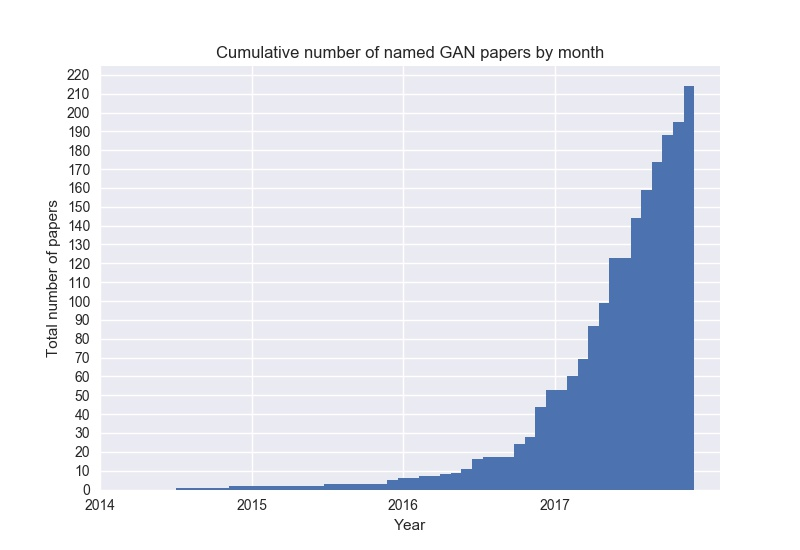
\includegraphics[scale=0.45]{cumulative_gans}
\caption{The cumulative amount of papers written about generative adversarial networks. The graph shows the exponential growth of GANs within the past three years. Image maintained by Avinash Hindipur \citep{November2017GANZoo}.}
\label{fig:CumulativeNumberofGANPapersbyMonth}
\end{figure}

\subsection{Fully Connected GANs}
The first generative adversarial network paper by Goodfellow \textit{et al.} made use of relatively simple fully connected neural networks for the generator and discriminator models. These are networks where each neuron in one layer is connected to every neuron in the following layer. This design is able to generate simple images and useful for proof of concept; however, several other architectures have overtaken this implementation \citep{2017arXiv171007035C}.

\subsection{Convolutional GANs}
Although convolutional neural networks (CNNs) seem well suited for the image generation tasks associated with GANs, difficulties associated with training initially constrained the use of convolutional models for both the discriminator and generator \citep{2017arXiv171007035C}. When implementing standard CNNs, one is often is unable to generate the same level of capacity and representational power. One solution proposed by Denton \textit{et al.} made use of Laplacian pyramids (LAPGAN), a type of image representation which repeatedly smooths and downsamples an image forming a sort of pyramid of images. At each layer of the pyramid, a conditional convolutional GAN is trained given generator output of the above layer. Another solution to this problem was proposed by Radford \textit{et al.}  simply made alterations to the existing deep convolutional network architecture \citep{2015arXiv151106434R}. Max pooling is replaced with strided layers within the discriminator and fractionally-strided layers within the generator. Furthermore, LeakyReLUs are used for all layers of the discriminator in place of the standard ReLU non-linearity function. The fractionally strided convolutions replicate within the generator replicate the benefits of the progressive upscaling within the Laplacian pyramid. The strided layers allow both the generator and discriminator to learn both the down-sampling and up-sampling operators during training \citep{2017arXiv171007035C}. Their architecture, called DCGAN, has become the base model for most GANs today \citep{2017arXiv170100160G}.

\subsection{Conditional GANs}
Initially proposed by Goodfellow as a straightforward extension of the first GAN architecture \citep{2014arXiv1406.2661G}, Mirza \textit{et al.} successfully implemented the conditional generative model in late 2014 \citep{2014arXiv1411.1784M}. Conditional generative models are constructed by feeding the additional parameter $\bm{c}$ to both to generator $G(\bm{z}|\bm{c})$ and discriminator $D(\bm{x}|\bm{c})$ to \textit{condition} the GAN. These architectures are better suited for multi-modal output \citep{2017arXiv171007035C}. By conditioning the GAN, it is possible to control the data generation process. These additional input may be class labels or other items such as text or an image. In section \ref{sec:img2img}, we will see how conditional GANs may be applied to image translation tasks. The new objective function of a conditional GAN becomes:

$$\min_{G}\max_{D}V(D, G) = \mathbb{E}_{x\sim p_{data}(x)}\Big[\log(D(\bm{x}|\bm{c}))\Big] + \mathbb{E}_{z\sim p_z(z)}\Big[\log(1-D(G(\bm{z}|\bm{c})))\Big]$$

\subsection{Inference GANs}
The first GAN architectures lacked methods to convert 

\subsection{Progressive GANs}

\section{Applications}
GANs are an exciting idea that are currently leading the frontier of deep generative models.
\subsection{Divergence Measures}
\subsection{Image Quality}
Hinton's Capsule Network
Progressive GANs
\subsection{Semi-Supervised Learning} \label{sec:semisupervised}
\subsection{Feature Learning}
\subsection{Semi-Supervised Learning}
\subsection{Reinforcement Learning}
\subsection{Image to Image Translation} \label{sec:img2img}


\section{Research Frontiers}
Evaluation, instability, mode collapse

Reinforcement learning

\section{Conclusion}
Generative models are currently being applied to many problems \citep{genmodelingopenai}; however, they offer many more possibilities due to their ability to understand the data they are given.

\bibliographystyle{plain}
\bibliography{references}
\end{document}
